% Auto-generated by generate_report.py — do not edit manually
% Preamble mirrors oxengthesis.cls so figures match the body text:
% Carlito as main font, Latin Modern Math via unicode-math.
\documentclass[border=6pt]{standalone}
\usepackage{fontspec}
\setmainfont{Carlito}
\usepackage{unicode-math}
\setmathfont{Latin Modern Math}
\usepackage{pgfplots}
\pgfplotsset{compat=1.18}
\usepgfplotslibrary{groupplots}
\usetikzlibrary{patterns,positioning}
\begin{document}
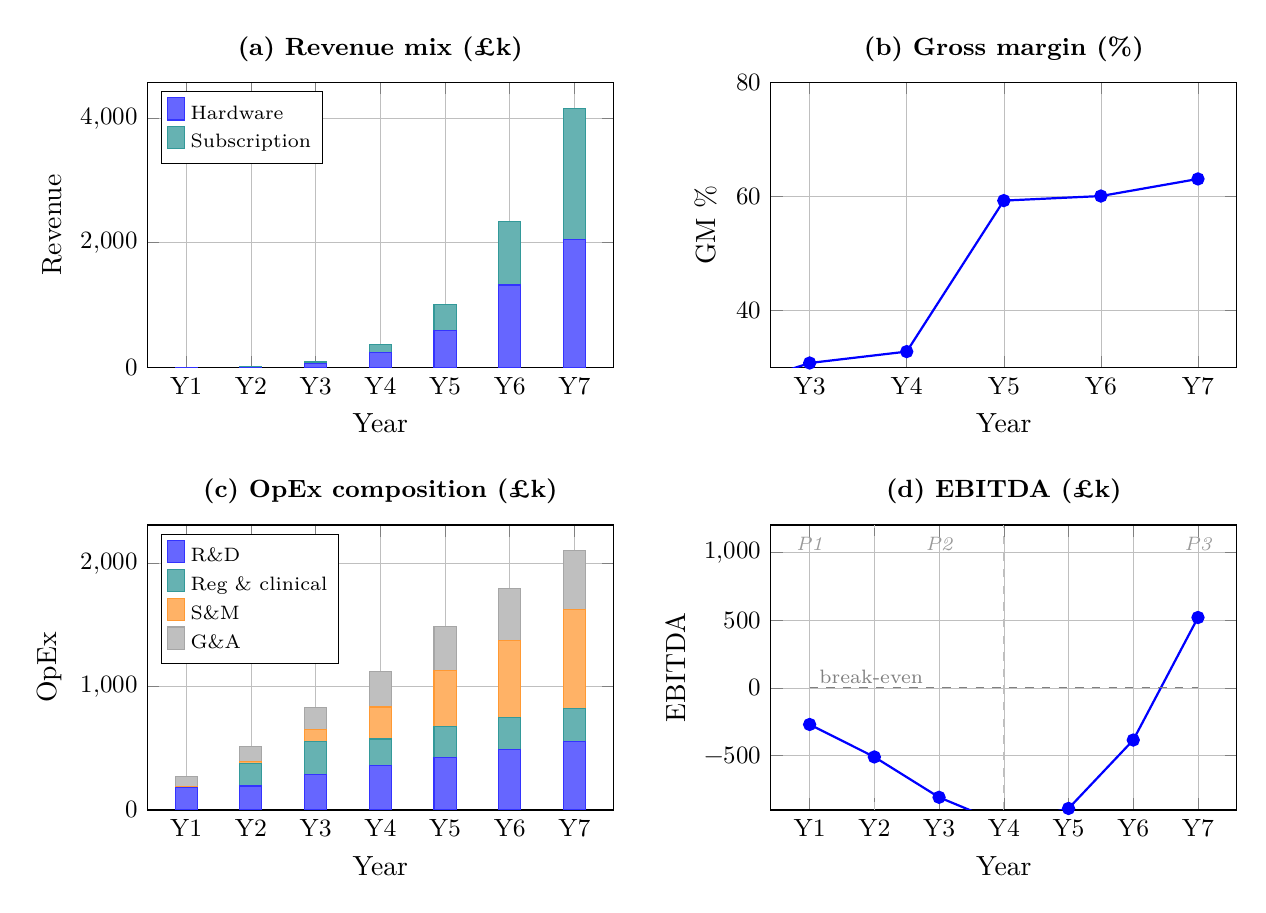
\begin{tikzpicture}
    \begin{groupplot}[
        group style={
            group size=2 by 2,
            horizontal sep=2.0cm,
            vertical sep=2.0cm,
        },
        width=7.5cm,
        height=5.2cm,
        symbolic x coords={Y1,Y2,Y3,Y4,Y5,Y6,Y7},
        xtick=data,
        xlabel={Year},
        grid=major,
        grid style={line width=.1pt, draw=gray!30},
        major grid style={line width=.2pt, draw=gray!50},
        tick label style={font=\small},
        label style={font=\normalsize},
        title style={font=\small\bfseries, yshift=-2pt},
        legend style={
            font=\scriptsize,
            cells={anchor=west},
            inner sep=2pt,
            row sep=-1pt,
        },
    ]

    % --- Panel (a): Revenue mix ---
    \nextgroupplot[
        title={(a) Revenue mix (\pounds k)},
        ylabel={Revenue},
        ybar stacked,
        bar width=8pt,
        ymin=0,
        legend pos=north west,
        legend columns=1,
    ]
    \addplot+[ybar,fill=blue!60,draw=blue!80] coordinates {(Y1,2.9) (Y2,7.3) (Y3,58.8) (Y4,235.2) (Y5,588.0) (Y6,1323.0) (Y7,2058.0)};
    \addplot+[ybar,fill=teal!60,draw=teal!80] coordinates {(Y1,1.1) (Y2,5.0) (Y3,30.2) (Y4,133.7) (Y5,422.7) (Y6,1022.3) (Y7,2093.1)};
    \legend{Hardware, Subscription}

    % --- Panel (b): Gross margin % ---
    \nextgroupplot[
        title={(b) Gross margin (\%)},
        ylabel={GM \%},
        ymin=30, ymax=80,
    ]
    \addplot[thick,blue,mark=*,mark size=2pt,mark options={solid,fill=blue}] coordinates {(Y1,12.5) (Y2,25.2) (Y3,30.8) (Y4,32.8) (Y5,59.3) (Y6,60.1) (Y7,63.1)};

    % --- Panel (c): OpEx composition ---
    \nextgroupplot[
        title={(c) OpEx composition (\pounds k)},
        ylabel={OpEx},
        ybar stacked,
        bar width=8pt,
        ymin=0,
        legend pos=north west,
        legend columns=1,
    ]
    \addplot+[ybar,fill=blue!60,draw=blue!80] coordinates {(Y1,184.0) (Y2,194.3) (Y3,286.8) (Y4,357.2) (Y5,422.7) (Y6,488.1) (Y7,553.6)};
    \addplot+[ybar,fill=teal!60,draw=teal!80] coordinates {(Y1,0.0) (Y2,185.5) (Y3,264.9) (Y4,218.6) (Y5,257.3) (Y6,262.3) (Y7,267.3)};
    \addplot+[ybar,fill=orange!60,draw=orange!80] coordinates {(Y1,5.3) (Y2,10.9) (Y3,104.0) (Y4,259.2) (Y5,454.2) (Y6,626.2) (Y7,801.7)};
    \addplot+[ybar,fill=gray!50,draw=gray!70] coordinates {(Y1,81.2) (Y2,121.8) (Y3,178.5) (Y4,291.1) (Y5,354.1) (Y6,417.1) (Y7,478.1)};
    \legend{R\&D, Reg \& clinical, S\&M, G\&A}

    % --- Panel (d): EBITDA trajectory with phase markers ---
    \nextgroupplot[
        title={(d) EBITDA (\pounds k)},
        ylabel={EBITDA},
        ymin=-900, ymax=1200,
    ]
    \draw[dashed,gray!50] (axis cs:Y2,-900) -- (axis cs:Y2,1200);
    \draw[dashed,gray!50] (axis cs:Y4,-900) -- (axis cs:Y4,1200);
    \node[anchor=north,font=\scriptsize\itshape,gray!80] at (axis cs:Y1,1180) {P1};
    \node[anchor=north,font=\scriptsize\itshape,gray!80] at (axis cs:Y3,1180) {P2};
    \node[anchor=north,font=\scriptsize\itshape,gray!80] at (axis cs:Y7,1180) {P3};
    \addplot[thick,blue,mark=*,mark size=2pt,mark options={solid,fill=blue}] coordinates {(Y1,-270.0) (Y2,-509.4) (Y3,-806.8) (Y4,-1005.3) (Y5,-889.0) (Y6,-384.7) (Y7,518.5)};
    \draw[dashed,gray,thin] (axis cs:Y1,0) -- (axis cs:Y7,0);
    \node[anchor=west,font=\scriptsize,gray] at (axis cs:Y1,80) {break-even};

    \end{groupplot}
\end{tikzpicture}

\end{document}
